% !TeX spellcheck = en_GB

\section{Monitor Pipeline}
\label{sec:concept:pipeline}

\begin{itemize}
	\item goal == monitor KNX traffic
	\item monitoring should include the whole network/world view
	\item monitoring needs to be distributed, so Line Couplers can be configured properly
	\item monitoring is done by agents
	\item agents will send data gather over a time window to the collector (ref to neflow terminology)
	\item time windows of agents are synchronised (by the collector) to make data analysis more reliable
	\item collector stores windows immediately in InfluxDB
	\item collector checks regularly the InfluxDB, if all agents send in their time window
	\item if so the collector relays all windows, describing the same time slot (+/- a couple seconds), to the analyser modules
	\item if not all windows are in by specified timeout (10s or so) they are relayed anyway
	\item bundled windows are distributed by pub-sub-server independently to different analytical modules
	\item analytical modules compare the windows to a base-line model (in different fashions)
\end{itemize}

\begin{figure}[h]
	\centering
	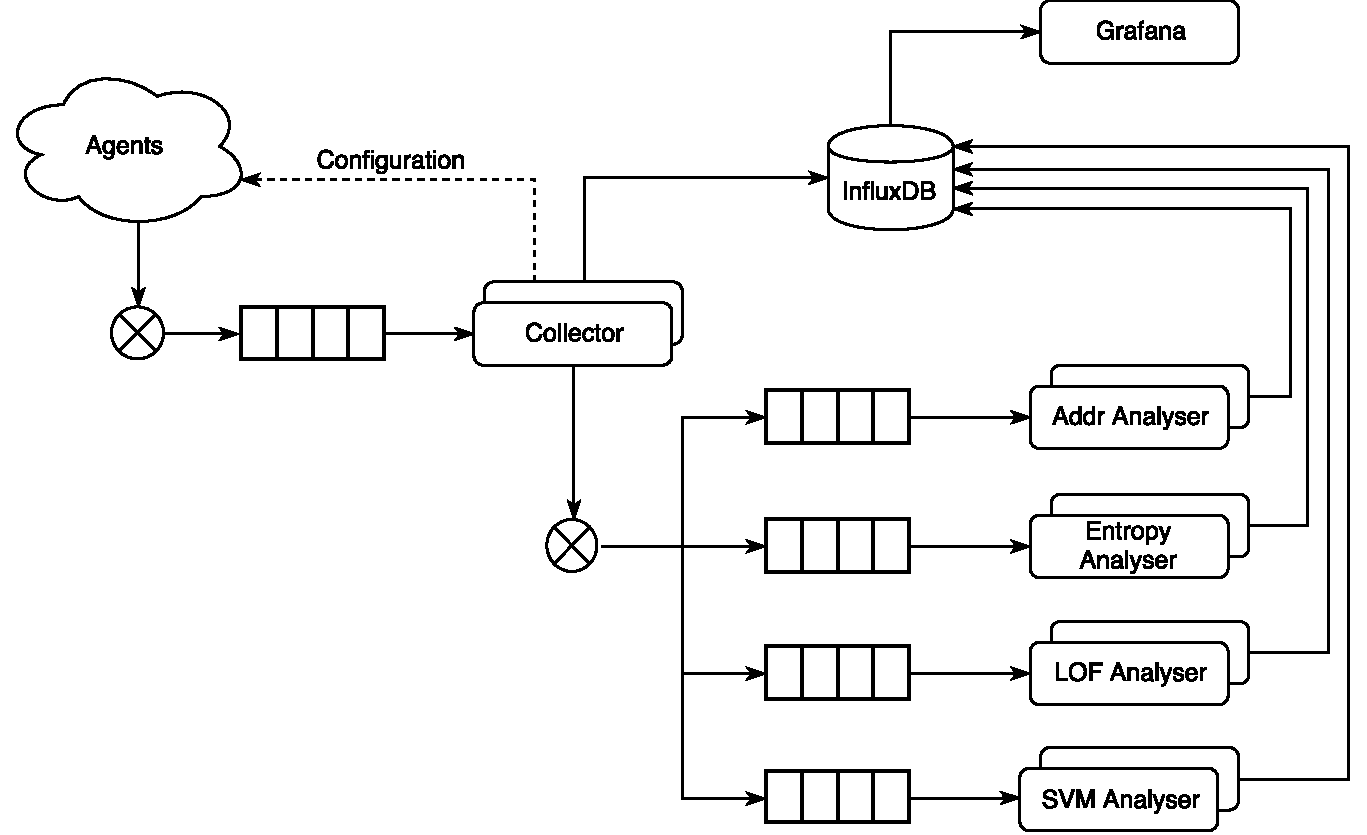
\includegraphics[width=\textwidth]{figures/300-concept-architecture.pdf}
	\caption[Pipeline Architecture]{Architecture of the monitoring pipeline}
	\label{fig:concept:architecture}
\end{figure}

\section{Design of Netflow Agent}
\label{sec:concept:agent}
cf. \textcite{Bloedorn2001} for a basic "How to get started" IDS Data Mining Infrastructure
\subsection{Truncating and Statistic Gathering}

\section{The Collector Module}
\label{sec:concept:collector}

\section{The Address Analyser}
\label{sec:concept:addr}

\section{The Local Outlier Factor Analyser}
\label{sec:concept:lof}

\section{The Entropy Analyser}
\label{sec:concept:entropy}

\section{Possible Errors and Design Drawbacks}
\label{sec:concept:flaws}
\begin{itemize}
	\item Errors in handling daylight saving time and time zones, due to missing time zone information in log
		\subitem simulated agent might be a bit off
		\subitem gap plus cummulated packets when daylight saving changes
\end{itemize}
